\documentclass[journal,12pt,twocolumn]{IEEEtran}
\usepackage{setspace}
\usepackage{gensymb}
\singlespacing
\usepackage[cmex10]{amsmath}
\usepackage{amsthm}
\usepackage{mathrsfs}
\usepackage{txfonts}
\usepackage{stfloats}
\usepackage{bm}
\usepackage{cite}
\usepackage{cases}
\usepackage{subfig}
\usepackage{longtable}
\usepackage{multirow}
\usepackage{enumitem}
\usepackage{mathtools}
\usepackage{steinmetz}
\usepackage{tikz}
\usepackage{circuitikz}
\usepackage{verbatim}
\usepackage{tfrupee}
\usepackage[breaklinks=true]{hyperref}
\usepackage{tkz-euclide}
\usetikzlibrary{calc,math}
\usepackage{listings}
    \usepackage{color}                                            %%
    \usepackage{array}                                            %%
    \usepackage{longtable}                                        %%
    \usepackage{calc}                                             %%
    \usepackage{multirow}                                         %%
    \usepackage{hhline}                                           %%
    \usepackage{ifthen}                                           %%
  %optionally (for landscape tables embedded in another document): %%
    \usepackage{lscape}     
\usepackage{multicol}
\usepackage{chngcntr}
\DeclareMathOperator*{\Res}{Res}
\renewcommand\thesection{\arabic{section}}
\renewcommand\thesubsection{\thesection.\arabic{subsection}}
\renewcommand\thesubsubsection{\thesubsection.\arabic{subsubsection}}

\renewcommand\thesectiondis{\arabic{section}}
\renewcommand\thesubsectiondis{\thesectiondis.\arabic{subsection}}
\renewcommand\thesubsubsectiondis{\thesubsectiondis.\arabic{subsubsection}}

% correct bad hyphenation here
\hyphenation{op-tical net-works semi-conduc-tor}
\def\inputGnumericTable{}                                 %%

\lstset{
frame=single, 
breaklines=true,
columns=fullflexible
}

\begin{document}


\newtheorem{theorem}{Theorem}[section]
\newtheorem{problem}{Problem}
\newtheorem{proposition}{Proposition}[section]
\newtheorem{lemma}{Lemma}[section]
\newtheorem{corollary}[theorem]{Corollary}
\newtheorem{example}{Example}[section]
\newtheorem{definition}[problem]{Definition}
\newcommand{\BEQA}{\begin{eqnarray}}
\newcommand{\EEQA}{\end{eqnarray}}
\newcommand{\define}{\stackrel{\triangle}{=}}

\bibliographystyle{IEEEtran}
\providecommand{\mbf}{\mathbf}
\providecommand{\pr}[1]{\ensuremath{\Pr\left(#1\right)}}
\providecommand{\qfunc}[1]{\ensuremath{Q\left(#1\right)}}
\providecommand{\sbrak}[1]{\ensuremath{{}\left[#1\right]}}
\providecommand{\lsbrak}[1]{\ensuremath{{}\left[#1\right.}}
\providecommand{\rsbrak}[1]{\ensuremath{{}\left.#1\right]}}
\providecommand{\brak}[1]{\ensuremath{\left(#1\right)}}
\providecommand{\lbrak}[1]{\ensuremath{\left(#1\right.}}
\providecommand{\rbrak}[1]{\ensuremath{\left.#1\right)}}
\providecommand{\cbrak}[1]{\ensuremath{\left\{#1\right\}}}
\providecommand{\lcbrak}[1]{\ensuremath{\left\{#1\right.}}
\providecommand{\rcbrak}[1]{\ensuremath{\left.#1\right\}}}
\theoremstyle{remark}
\newtheorem{rem}{Remark}
\newcommand{\sgn}{\mathop{\mathrm{sgn}}}
\providecommand{\abs}[1]{\left\vert#1\right\vert}
\providecommand{\res}[1]{\Res\displaylimits_{#1}} 
\providecommand{\norm}[1]{\left\lVert#1\right\rVert}
\providecommand{\mtx}[1]{\mathbf{#1}}
\providecommand{\mean}[1]{E\left[ #1 \right]}
\providecommand{\fourier}{\overset{\mathcal{F}}{ \rightleftharpoons}}
\providecommand{\system}{\overset{\mathcal{H}}{ \longleftrightarrow}}
\newcommand{\solution}{\noindent \textbf{Solution: }}
\newcommand{\cosec}{\,\text{cosec}\,}
\providecommand{\dec}[2]{\ensuremath{\overset{#1}{\underset{#2}{\gtrless}}}}
\newcommand{\myvec}[1]{\ensuremath{\begin{pmatrix}#1\end{pmatrix}}}
\newcommand{\mydet}[1]{\ensuremath{\begin{vmatrix}#1\end{vmatrix}}}
\numberwithin{equation}{subsection}
\makeatletter
\@addtoreset{figure}{problem}
\makeatother

\let\StandardTheFigure\thefigure
\let\vec\mathbf
\renewcommand{\thefigure}{\theproblem}



\def\putbox#1#2#3{\makebox[0in][l]{\makebox[#1][l]{}\raisebox{\baselineskip}[0in][0in]{\raisebox{#2}[0in][0in]{#3}}}}
     \def\rightbox#1{\makebox[0in][r]{#1}}
     \def\centbox#1{\makebox[0in]{#1}}
     \def\topbox#1{\raisebox{-\baselineskip}[0in][0in]{#1}}
     \def\midbox#1{\raisebox{-0.5\baselineskip}[0in][0in]{#1}}

\vspace{3cm}


\title{Assignment 1}
\author{Jaswanth Chowdary Madala}





% make the title area
\maketitle

\newpage

%\tableofcontents

\bigskip

\renewcommand{\thefigure}{\theenumi}
\renewcommand{\thetable}{\theenumi}


\begin{enumerate}
\item Two congruent circles intersect each other at points $\vec{A}$ and $\vec{B}$. Through $\vec{A}$ any line segment $\vec{PAQ}$ is drawn so that $\vec{P}$, $\vec{Q}$ lie on the two circles. Prove that $\vec{BP} = \vec{BQ}$.
\begin{figure}[ht]
\centering
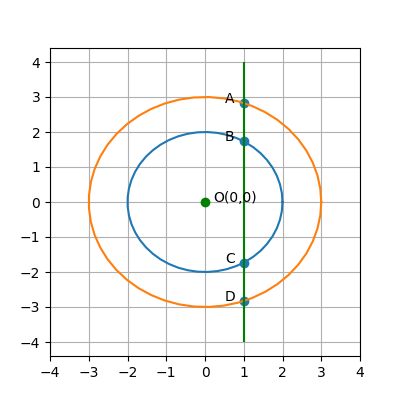
\includegraphics[width = \columnwidth]{"./figs/fig.png"}
\caption{Graph}
\label{fig:1}
\end{figure}

\textbf{Solution:}
Consider two congruent circles with radius $2\sqrt{2}$ with centres at \brak{2,0}, \brak{-2,0}. The equations of these circles is given by,
\begin{align}
\norm{\vec{x}}^2 + 2\vec{u_1}^\top\vec{x} + f_1 &= 0 
\label{eq0}\\
\norm{\vec{x}}^2 + 2\vec{u_2}^\top\vec{x} + f_2 &= 0 
\label{eq1}\\
\vec{u_1} = -\myvec{2\\0}, \, \vec{u_2} &= -\myvec{-2\\0}\\
f_1 = -4, \, f_2 &= -4
\end{align}
To get points of intersection $\vec{A}, \vec{B}$
\begin{align}
\norm{\vec{x}}^2 + 2\vec{u_1}^\top\vec{x} + f_1 &= \norm{\vec{x}}^2 + 2\vec{u_2}^\top\vec{x} + f_2\\
2\brak{\vec{u_1}-\vec{u_2}}^\top\vec{x} &= f_2 - f_1\\
2\myvec{-4&0}\vec{x} &= 0\\
\vec{x} &= \myvec{\alpha\\\beta}\\
\alpha &= 0\\
\vec{x} &= \myvec{0 \\ \beta}
\label{eq2}
\end{align}
Substituting \eqref{eq2} in \eqref{eq0} we get,
\begin{align}
\beta^2 - 2\myvec{2&0}\myvec{0\\\beta}-4 &= 0\\
\beta^2 &= 4\\
\beta &= \pm 2\\
\vec{A} = \myvec{0\\2}, \, \vec{B} &= \myvec{0\\-2}
\end{align}
Equation of the line passing through $\vec{A}$ is given by
\begin{align}
\vec{n}^\top \vec{x} = \vec{n}^\top \vec{A}
\end{align}
Let the noRmal vector $\vec{n}$ given by,
\begin{align}
\vec{n} &= \myvec{2\\1}\\
\myvec{2&1}\vec{x} &= \myvec{2&1}\myvec{0\\2}\\
\myvec{2&1}\vec{x} &= 2
\label{eq3}
\end{align}
Let $\vec{P}$ be the intersection of the line \eqref{eq3} and the circle \eqref{eq0}, $\vec{Q}$ be the intersection of the line \eqref{eq3} and the circle \eqref{eq1}. 
\begin{align}
\vec{P} = \myvec{x_1\\y_1}, \, \vec{Q} &= \myvec{x_2\\y_2}\\
2x_1 + y_1 &= 2\\
2x_2 + y_2 &= 2
\end{align}
To find the point $\vec{P}$,
\begin{align}
y_1 &= 2 - 2x_1\\
x_1^2 + y_1^2 - 2\myvec{2&0}\myvec{x_1\\y_1}-4 &= 0\\
x_1^2 + y_1^2 - 4 x_1-4 &= 0\\
x_1^2 + \brak{2-2x_1}^2 -4x_1 -4 &= 0\\
5x_1^2 - 12x_1 &= 0\\
x_1 &= 0, \frac{12}{5}\\
\vec{P} &= \myvec{\frac{12}{5}\\\\-\frac{14}{5}}
\end{align}

To find the point $\vec{Q}$,
\begin{align}
y_2 &= 2 - 2x_2\\
x_2^2 + y_2^2 - 2\myvec{-2&0}\myvec{x_2\\y_2}-4 &= 0\\
x_2^2 + y_2^2 +4 x_2-4 &= 0\\
x_2^2 + \brak{2-2x_2}^2 +4x_2 -4 &= 0
\end{align}

\begin{align}
5x_2^2 -4x_2&= 0\\
x_2 &= 0,\frac{4}{5}\\
\vec{Q} &= \myvec{\frac{4}{5}\\\\\frac{2}{5}}
\end{align}
\begin{align}
\norm{\vec{BP}} &= \norm{\myvec{0\\\\-2} - \myvec{\frac{12}{5}\\\\-\frac{14}{5}}}\\
&= \norm{\myvec{-\frac{12}{5}\\\\\frac{4}{5}}}\\
&= \frac{4\sqrt{10}}{5}\\
\norm{\vec{BQ}} &= \norm{\myvec{0\\\\-2} - \myvec{\frac{4}{5}\\\\\frac{2}{5}}}\\
&= \norm{\myvec{-\frac{4}{5}\\\\-\frac{12}{5}}}\\
&= \frac{4\sqrt{10}}{5}
\end{align}
Hence, $\vec{BP} = \vec{BQ}$.
\end{enumerate}
\end{document}



